\section{Results}
\label{sec:results-v2}
SCIT-Speech represented speech as a 1.5-kbit/s stream of shared-codebook indices and used that same payload for waveform reconstruction and receiver-side speaker identification. We evaluated these capabilities at a fixed three-layer residual vector quantization (RVQ) operating point, $L=3$, corresponding to approximately 170-fold compression relative to 16-kHz, 16-bit mono pulse-code modulation (PCM). The evidence addresses five linked questions: how the payload is formed, how much computation its encoder requires, how well it reconstructs speech against rate-matched codecs, how reconstruction changes under index-domain perturbations, and whether the frozen representation retains information sufficient to distinguish speakers. Reconstruction comparisons used 300 LibriSpeech test-clean utterances; robustness used all 2,620 test-clean utterances; and identification used a separate, locked 110-speaker VCTK protocol. These populations and endpoints are reported separately.

\subsection{Shared codebooks reduce the speech payload to 1.5 kbit/s}
\label{sec:rv2-payload}
The transmission rate was determined by discrete codebook choices rather than by the dimensionality of the speech features. Following the SpeechTokenizer framework~\cite{speechtokenizer}, the encoder mapped mono 16-kHz audio to 1024-dimensional latent frames at 50~Hz. Three residual quantizers successively represented each frame with one entry from each of three 1024-entry codebooks. The channel carried only the resulting integer indices; model weights and codebook vectors remained locally stored. At the receiver, lookup and summation recovered the quantized representation for waveform decoding (Fig.~\ref{fig:rv2-components}). Thus, the transmitter did not send a 1024-dimensional vector for every latent frame.

\begin{figure*}[t]
\centering
\setlength{\tabcolsep}{3pt}
\begin{tabular}{c c c c c c c}
\fbox{\parbox[c][1.15cm][c]{0.18\textwidth}{\centering 16-kHz speech\\NAS encoder\\1024-D frames, 50 Hz}}
&$\rightarrow$&
\fbox{\parbox[c][1.15cm][c]{0.18\textwidth}{\centering Shared RVQ\\3 codebooks\\1024 entries each}}
&$\rightarrow$&
\fbox{\parbox[c][1.15cm][c]{0.18\textwidth}{\centering Index payload\\150 indices/s\\10 bits/index}}
&$\rightarrow$&
\fbox{\parbox[c][1.15cm][c]{0.18\textwidth}{\centering Local codebooks\\Waveform decoder\\Reconstructed speech}}
\end{tabular}
\par\medskip
\begin{tabular}{c c c c c}
\parbox[c]{0.38\textwidth}{\centering Received indices $\widetilde I$ $\rightarrow$ Token encoder\\[3pt]
Reconstructed speech $\hat{x}$ $\rightarrow$ Frozen ECAPA-TDNN\\and trainable audio projection}
&$\rightarrow$&
\fbox{\parbox[c][1cm][c]{0.18\textwidth}{\centering Gated embedding\\fusion}}
&$\rightarrow$&
\fbox{\parbox[c][1cm][c]{0.18\textwidth}{\centering Closed-set\\110-speaker classifier}}
\end{tabular}
\caption{One index payload supports reconstruction and identification. The upper path shows the fixed $L=3$ codec interface. All reconstruction comparisons use the NAS-selected encoder. The lower path uses received indices and their matching reconstruction from frozen SCIT-LCA; classifier training does not update the speech codec or the ECAPA backbone. The token encoder, audio projection and fusion classifier are trained at the receiver. No separate identity embedding is transmitted. This diagram specifies the evaluated deep-learning components, not a completed multi-user transport experiment.}
\label{fig:rv2-components}
\end{figure*}

The fixed-length index budget follows directly from this interface. With $f_q=50$ latent frames per second, $K=1024$ entries per codebook and $L=3$ retained layers,
\begin{equation}
\begin{aligned}
R_{\rm index}
 &=Lf_q\lceil\log_2 K\rceil\\
 &=3\times50\times10=1500\ {\rm bit/s}.
\end{aligned}
\label{eq:rv2-rate}
\end{equation}
Compared with $16{,}000\times16=256{,}000$~bit/s PCM, this yields a nominal compression ratio of $256{,}000/1500=170.7$. It is an index-only rate, not a measurement of total network traffic. For example, a 0.5-s block contains 25 latent frames and 75 indices, requiring 750 bits or 94 bytes after final-byte padding. The resulting 1504-bit/s byte-aligned payload still excludes headers, transport framing and security overhead. The codec comparisons below use the nominal 1.5-kbit/s operating point consistently.

Let $\widetilde I_{m,t}$ denote the index available to the receiver for quantizer $m$ and frame $t$. Using the corresponding local codebooks $C_m$, reconstruction is
\begin{equation}
\hat z_t=\sum_{m=1}^{3} C_m[\widetilde I_{m,t}],
\qquad \hat x=D_\phi(\hat Z).
\label{eq:rv2-reconstruction}
\end{equation}
Under clean transmission, these are the original encoder-selected indices. In the robustness tests, the same interface accepts perturbed indices without transmitting extra features. The speaker module likewise reads the received indices and the waveform decoded from them, so its additional computation does not require an additional identity payload. This receiver-side reuse is distinct from inserting a watermark or an explicit biometric identifier.

The representation was trained to support reconstruction while retaining semantic information. The base codec combined waveform and multi-scale mel reconstruction losses, adversarial and feature-matching objectives, RVQ commitment, and supervision of the first RVQ layer by frozen HuBERT features~\cite{hubert}. Semantic supervision did not enforce a strict partition between linguistic content and speaker cues. We therefore evaluated reconstruction and identification separately instead of assuming that either follows from the other. The fixed $L=3$ setting defines all quantitative comparisons in this Results section; training-time layer sampling is described below only where needed to interpret channel adaptation.

\subsection{Architecture search lowers encoder cost while preserving the codec interface}
\label{sec:rv2-nas}
The selected encoder reduced both storage and arithmetic cost without changing the number of transmitted indices. Neural architecture search (NAS) varied encoder width, stride arrangement, recurrent depth, activation and residual operators while holding the total downsampling factor at 320 and the latent dimension at 1024. These interface constraints preserved the 50-Hz frame rate and allowed candidate encoders to be assessed against the same pretrained SpeechTokenizer teacher. The codebooks and decoder were not part of the architecture search.

The search profiled 8,192 configuration candidates, then successively retained 512, 64 and eight candidates for short teacher-alignment runs of 100, 500 and 1,500 steps. Candidate encoders were trained to match the frozen teacher's pre-quantization features using latent distance, cosine agreement and temporal-difference objectives. Ranking combined these alignment and reconstruction proxies with parameter, multiply--accumulate operation (MAC) and real-time factor (RTF) costs. The final architecture minimized the combined score among nondominated candidates. Selection therefore represented a quality--resource trade-off, not the minimum-parameter architecture in the search space.

\begin{figure*}[t]
\centering
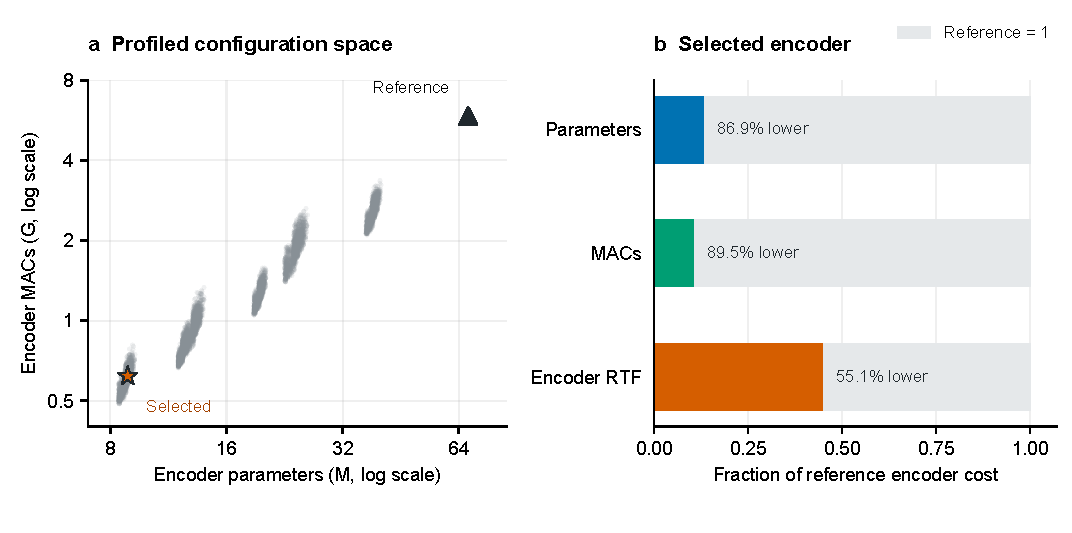
\includegraphics[width=\textwidth]{results_v2_assets/nas_resources.pdf}
\caption{Encoder resource reduction at the preserved latent interface. \textbf{a}, Initial-stage profiles of 8,192 configuration candidates, with the hand-designed reference marked by a triangle and the subsequently selected encoder by a star. Points can overlap; configuration count is not a claim that all networks are structurally distinct. Both axes are logarithmic. This panel shows resource profiles, not a quality Pareto frontier. \textbf{b}, Selected-encoder costs normalized to the reference. RTF is encoder-only FP32 inference on an RTX 5070 Ti for a one-second input, averaged over five synchronized passes. The profiles exclude RVQ, decoding, speaker inference and transport.}
\label{fig:rv2-nas}
\end{figure*}

The selected architecture used a $(5,4,4,4)$ stride schedule, 24 initial filters, one bidirectional LSTM layer and Snake activation. Relative to the hand-designed reference, its parameter count fell from 67.706~M to 8.873~M, a reduction of 86.9\%, and MACs fell from 5.869~G to 0.618~G, a reduction of 89.5\% (Fig.~\ref{fig:rv2-nas}). The initial-stage encoder RTF decreased from 0.00819 to 0.00368, or by 55.1\%. These resource measurements describe the sender-side encoder only; they do not imply an equivalent reduction for the complete codec or the receiver-side identity module.

The short-run scores served architecture selection rather than held-out quality estimation. Proxy training and scoring reused small, nested subsets of eight, 16 and 32 training utterances. They could identify compatible, computationally economical encoders, but could not establish final reconstruction quality or generalization by themselves. Only the selected architecture was carried forward. The NAS encoder, RVQ codebooks and decoder were then trained jointly from scratch to form the base codec, hereafter SCIT.

This separation also distinguishes two forms of supervision in the pipeline. Search-time distillation matched the pretrained SpeechTokenizer encoder's 1024-dimensional, pre-RVQ representation while its downstream modules remained frozen. Subsequent codec training used 768-dimensional HuBERT targets to guide the first quantizer, alongside reconstruction and adversarial learning. It did not reuse a short-trained search checkpoint as the final codec. Codec training used 27,039 LibriSpeech train-clean-100 utterances with a disjoint 1,500-utterance validation set; validation mel loss selected the retained SCIT checkpoint. Neither reconstruction test population was used for this training.

All subsequent SCIT and SCIT-LCA measurements therefore use the lightweight architecture, but the external-codec comparison is a comparison of complete trained systems. It does not isolate the contribution of NAS from the training objectives or other codec components. Similarly, the measured encoder RTF is not end-to-end latency: bidirectional recurrence and noncausal convolutions require buffered inference in the implemented block interface. The results establish a substantially lower encoder resource requirement under the recorded profiling conditions, followed by separate tests of the resulting codec's reconstruction capability.

\subsection{The 1.5-kbit/s codec outperforms rate-matched baselines on objective reconstruction scores}
\label{sec:rv2-quality}
SCIT reconstructed held-out speech more accurately than the evaluated DAC and EnCodec operating points at the same nominal rate. The comparison used the first 300 utterances in the retained LibriSpeech test-clean manifest, with each waveform processed in full and each utterance receiving equal weight. The pretrained 16-kHz DAC baseline used three active quantizers~\cite{dac}; the pretrained 24-kHz EnCodec baseline used its 1.5-kbit/s setting~\cite{encodec}, with resampling before encoding and after decoding. Neither external model was fine-tuned on the evaluation subset.

\begin{table*}[t]
\centering
\caption{Clean-channel reconstruction on 300 LibriSpeech test-clean utterances. Entries are means [95\% utterance-bootstrap intervals]. The first three codecs share the nominal 1.5-kbit/s operating point; bold means identify the best in that group. Opus and PCM are higher-rate references. Lower mel-L1 and higher STOI/PESQ-WB are better.}
\label{tab:rv2-quality}
\small\setlength{\tabcolsep}{5pt}
\begin{tabular}{lrrrr}
\toprule
Codec & kbit/s & mel-L1 & STOI & PESQ-WB\\
\midrule
SCIT & 1.5 & \textbf{0.864} [0.855, 0.874] & \textbf{0.892} [0.889, 0.895] & \textbf{2.097} [2.067, 2.128]\\
DAC ($n_q=3$) & 1.5 & 1.232 [1.219, 1.245] & 0.799 [0.796, 0.803] & 1.284 [1.266, 1.303]\\
EnCodec & 1.5 & 1.282 [1.266, 1.297] & 0.848 [0.845, 0.851] & 1.612 [1.585, 1.638]\\
Opus & 6.0 & 2.302$^\dagger$ [2.275, 2.330] & 0.906 [0.903, 0.908] & 2.237 [2.187, 2.287]\\
PCM & 256 & 0.000 [0.000, 0.000] & 1.000 [1.000, 1.000] & 4.644 [4.644, 4.644]\\
\bottomrule
\end{tabular}
\par\smallskip
\parbox{\textwidth}{\footnotesize $^\dagger$Full-band mel-L1 is sensitive to low-rate Opus bandwidth reduction and is not a standalone cross-codec perceptual ranking. Intervals use 10,000 resamples and seed 42; displayed values are rounded to three decimals.}
\end{table*}


We evaluated three complementary, reference-based quantities: log-mel spectral error (mel-L1), short-time objective intelligibility (STOI)~\cite{stoi}, and wideband perceptual evaluation of speech quality (PESQ-WB)~\cite{pesq}. All reference and reconstructed signals were compared as mono 16-kHz audio after trimming to their common length, without an additional time-alignment optimization. Mel-L1 was a single-scale evaluation metric, distinct from the weighted multi-scale training loss. Table~\ref{tab:rv2-quality} reports utterance means and archived 95\% bootstrap intervals, allowing spectral error, predicted intelligibility and predicted perceptual quality to be read together.

At 1.5~kbit/s, SCIT achieved STOI 0.892, compared with 0.799 for DAC and 0.848 for EnCodec. Its PESQ-WB was 2.097, compared with 1.284 and 1.612, respectively. The mel-L1 ordering agreed: SCIT obtained 0.864, versus 1.232 for DAC and 1.282 for EnCodec. Thus, the advantage was not confined to one of the three reported metrics. On the displayed precision, the STOI gains were 0.093 over DAC and 0.044 over EnCodec, with corresponding PESQ-WB gains of 0.813 and 0.485.

The per-codec confidence intervals did not overlap between SCIT and either matched-rate baseline for any of these metrics. Those intervals summarize resampling variation over this 300-utterance evaluation population, not variation across independently trained codec instances or a paired significance test. The result supports a consistent objective-score advantage for the evaluated checkpoints and settings. It does not establish superiority over every possible configuration of either baseline, and the systematic manifest subset should not be treated as an independent random sample of all speech conditions.

The higher-rate Opus reference provides a different comparison. At a requested 6~kbit/s, four times the nominal SCIT rate, Opus achieved STOI 0.906 and PESQ-WB 2.237. SCIT was therefore close in STOI, with a gap of 0.014, but did not match Opus on both objective scores. This is a useful bitrate--quality comparison rather than evidence of perceptual equivalence. The PCM passthrough row supplies the same-metric reference at 256~kbit/s; its zero spectral error and unit STOI also distinguish compressed reconstruction from lossless transmission.

Opus additionally illustrates why the metrics must not be collapsed into a single ranking without qualification. Its full-band mel-L1 was higher despite its better STOI and PESQ-WB, reflecting the sensitivity of that spectral metric to low-rate bandwidth reduction. We therefore interpret mel-L1 alongside the other measures. Together, the measurements show that the compact SCIT payload preserves information useful for objective intelligibility and reconstruction quality; they do not constitute a listening study, a word-error-rate assessment, or an evaluation of block-streaming audio. The next comparison asks whether these benefits persist when the indices available to the decoder are perturbed.

\subsection{Channel adaptation improves index-error tolerance with a metric-dependent trade-off}
\label{sec:rv2-robustness}
Channel-aware fine-tuning improved mel-L1 and STOI in every reported condition, but did not improve PESQ-WB uniformly. Starting from SCIT, the adapted codec, SCIT-LCA, retained the same architecture, codebook sizes and nominal rate. Its communication branch sampled clean indices, 5\% or 10\% index erasure, or 1\% or 3\% index substitution, together with training-time sampling of the retained RVQ depth. Reconstruction and clean--perturbed consistency losses supplemented the base objective. The retained checkpoint was selected by validation communication-branch mel loss, not by any test perturbation score.

The distinction between training augmentation and evaluation is important here. Independent index errors were included during fine-tuning; packet-wise and burst masks were additional stress tests, not additional training augmentations. We evaluated all conditions at $L=3$ on all 2,620 LibriSpeech test-clean utterances. SCIT and SCIT-LCA used matched utterances and matched perturbation seeds. The full-set means in Table~\ref{tab:rv2-robustness} are therefore not interchangeable with the 300-utterance external-codec means in Table~\ref{tab:rv2-quality}.

\begin{table*}[t]
\centering
\caption{SCIT and SCIT-LCA on all 2,620 LibriSpeech test-clean utterances at $L=3$. Means are computed from paired utterances with matched perturbation seeds. Bold entries indicate the favourable direction within each condition, not statistical significance. Erasure and packet/burst masks use the previous original index, with the first frame protected.}
\label{tab:rv2-robustness}
\small\setlength{\tabcolsep}{6pt}
\begin{tabular}{lrrrrrr}
\toprule
& \multicolumn{2}{c}{mel-L1 $\downarrow$} & \multicolumn{2}{c}{STOI $\uparrow$} & \multicolumn{2}{c}{PESQ-WB $\uparrow$}\\
\cmidrule(lr){2-3}\cmidrule(lr){4-5}\cmidrule(lr){6-7}
Condition & SCIT & SCIT-LCA & SCIT & SCIT-LCA & SCIT & SCIT-LCA\\
\midrule
Clean & 0.9075 & \textbf{0.8711} & 0.8853 & \textbf{0.8922} & \textbf{1.9538} & 1.9397\\
10\% index erasure & 0.9986 & \textbf{0.9511} & 0.8457 & \textbf{0.8580} & 1.5364 & \textbf{1.5549}\\
3\% index substitution & 0.9716 & \textbf{0.9266} & 0.8640 & \textbf{0.8723} & 1.7027 & \textbf{1.7150}\\
5\% packet loss (100 ms) & 0.9336 & \textbf{0.8959} & 0.8727 & \textbf{0.8805} & \textbf{1.8096} & 1.8067\\
One 200-ms burst & 0.9271 & \textbf{0.8902} & 0.8752 & \textbf{0.8826} & \textbf{1.8674} & 1.8584\\
\bottomrule
\end{tabular}
\par\smallskip
\parbox{\textwidth}{\footnotesize The burst condition removes one randomly placed span of ten latent frames per utterance; it is not a fixed percentage of packet loss. These token-domain perturbations do not emulate a complete packet-loss concealment receiver.}
\end{table*}


On the full clean set, SCIT-LCA reduced mel-L1 from 0.9075 to 0.8711 and increased STOI from 0.8853 to 0.8922. PESQ-WB, however, decreased from 1.9538 to 1.9397, a difference of $-0.0141$. Adaptation thus produced a modest clean-channel trade-off rather than an improvement in every aspect of reconstruction. Reporting the absolute scores makes this distinction visible and prevents the small PESQ decrease from being hidden by the favourable directions of the other two metrics.

The clearest extension of the adaptation benefit occurred under independent index errors. At 10\% erasure, SCIT-LCA increased STOI from 0.8457 to 0.8580 and reduced mel-L1 from 0.9986 to 0.9511. The mel-L1 difference, $-0.0475$, was larger in magnitude than the clean-channel difference of $-0.0364$; the STOI difference likewise increased from 0.0069 to 0.0123. PESQ-WB changed direction relative to the clean comparison, increasing from 1.5364 to 1.5549. Under 3\% substitution, SCIT-LCA also improved all three means: mel-L1 decreased by 0.0451, STOI increased by 0.0082 and PESQ-WB increased by 0.0122. These conditions directly test the discrete-index perturbations represented during adaptation.

Both codecs nevertheless degraded relative to their own clean outputs. For example, SCIT-LCA's STOI fell from 0.8922 to 0.8580 under 10\% erasure, and its PESQ-WB fell from 1.9397 to 1.5549. The adaptation advantage is therefore partial resilience, not correction of every corrupted index or preservation of clean-channel quality. Moreover, the erasure and substitution probabilities describe different perturbation processes; their absolute scores are not a controlled ranking of channel severity at a shared error budget.

For temporally grouped masks, a packet comprised five latent frames, or 100~ms, and was selected for masking with probability 5\% across all three layers. The burst condition masked one randomly placed span of ten frames, or 200~ms, per utterance. Under the packet condition, SCIT-LCA improved STOI from 0.8727 to 0.8805 and reduced mel-L1 from 0.9336 to 0.8959. Under the burst condition, the corresponding scores changed from 0.8752 to 0.8826 and from 0.9271 to 0.8902. PESQ-WB remained slightly below SCIT in both cases, by 0.0030 and 0.0090, respectively. The favourable mel-L1 and STOI directions therefore extended beyond the independent-error augmentations, while the PESQ benefit did not.

These grouped-mask results have a specific implementation boundary. Masked positions copied the preceding original index, with the first frame protected; consecutive losses did not recursively reuse the last successfully received index. The experiments consequently measure sensitivity to the implemented token-domain perturbations, not a deployable packet-loss concealment strategy. A single 200-ms span also represents a duration-dependent fraction of each utterance, rather than a fixed packet-loss percentage. Within those conditions, the absolute means establish a consistent spectral-error and STOI benefit and a smaller, condition-dependent PESQ change. They do not demonstrate network-level error recovery, statistical equivalence between codecs, or speaker-identification robustness under corrupted transmission.

\begin{table*}[t]
\centering
\caption{Closed-set speaker identification from a frozen SCIT-LCA payload ($L=3$, 110 speakers, 1,650 test utterance groups). All entries are percentages. Mean $\pm$ SD uses the sample standard deviation across three training seeds. Worst 10\% is the mean accuracy of the 11 lowest-accuracy speakers. The last column reports within-seed hierarchical-bootstrap intervals, not uncertainty on the three-seed mean.}
\label{tab:rv2-speaker}
\small\setlength{\tabcolsep}{5pt}
\begin{tabular}{lrrrrrr}
\toprule
Seed & Top-1 & Macro-F1 & Top-5 & ECE & Worst 10\% & Top-1 95\% CI\\
\midrule
41 & 95.03 & 94.94 & 99.39 & 1.30 & 76.97 & [93.21, 96.73]\\
42 (delivery) & 94.18 & 94.14 & 99.27 & 2.04 & 73.94 & [92.12, 95.88]\\
43 & 95.58 & 95.56 & 99.39 & 1.92 & 82.42 & [94.00, 97.03]\\
\textbf{Mean} & \textbf{94.93 $\pm$ 0.70} & \textbf{94.88 $\pm$ 0.71} & \textbf{99.35} & \textbf{1.75} & \textbf{77.78} & --\\
\bottomrule
\end{tabular}
\par\smallskip
\parbox{\textwidth}{\footnotesize Seed 42 was predeclared for delivery. Intervals are retained from the archived analysis; its bootstrap replicate count and RNG seed remain an author-confirmation item in Methods and Supplementary Methods S7.}
\end{table*}


\subsection{A frozen 1.5-kbit/s payload supports accurate closed-set speaker identification}
\label{sec:rv2-speaker}
The same low-rate representation retained speaker information that a receiver-side classifier could recover without modifying the codec. For this experiment, SCIT-LCA was frozen at $L=3$, and its full-utterance indices and reconstructed waveforms were cached before classifier training. Codec state hashes matched before and after caching, and codec parameters were excluded from classifier optimization. The measured identification performance therefore arose from learning to read an existing representation, not from allocating extra bits or retuning the speech codec for speaker labels.

The receiver combined two views of that representation (Fig.~\ref{fig:rv2-components}). A token branch embedded the three RVQ index sequences and used temporal residual blocks and attentive statistics pooling to form a 256-dimensional speaker embedding. An audio branch applied pretrained ECAPA-TDNN~\cite{ecapa} to reconstructed speech and projected its output to the same dimension. The ECAPA backbone remained frozen throughout the reported runs; codec-aware adaptation concerned the projection and classifier, not backbone fine-tuning. An element-wise gate fused the two embeddings, with additive angular-margin objectives for the fusion and auxiliary branch heads~\cite{arcface}. Only the fusion head was used for test prediction. Both inputs were available from the same received speech payload.

Evaluation used 110 speakers from the microphone-1 recordings of VCTK 0.92~\cite{vctk}. A canonical split allocated 80, 15 and 15 utterance groups per speaker to training, validation and test, respectively, giving 8,800 training, 1,650 validation and 1,650 test items. Utterance groups did not overlap, but speaker identities were shared across splits, as required by closed-set identification. Matched token/audio crops covered up to three seconds; validation and test used deterministic centre crops and all three RVQ layers. The primary split was not globally transcript-disjoint, so it did not by itself isolate speaker cues from all lexical regularities.

Three runs with seeds 41, 42 and 43 used the same split. Validation macro-F1 selected checkpoints, and validation data alone fitted each run's scalar temperature for probability calibration. Each frozen configuration was evaluated once on the locked test set. Seed 42 was declared in advance as the delivery checkpoint rather than selected retrospectively for its test accuracy. This protocol separates model selection, confidence calibration and final measurement while exposing training-seed variability.

Across the three runs, mean Top-1 accuracy was $94.93\%\pm0.70\%$ and mean macro-F1 was $94.88\%\pm0.71\%$, where the variation is the sample standard deviation across training seeds (Table~\ref{tab:rv2-speaker}). Mean Top-5 accuracy was 99.35\%. The individual Top-1 results ranged from 94.18\% to 95.58\%, far above the $1/110\approx0.91\%$ uniform-guessing reference. These measurements establish that a fixed low-rate codec can support high-accuracy identification among the enrolled classes even though it was not updated during classifier training.

The archived hierarchical-bootstrap intervals provide a separate view of within-seed uncertainty. They resampled speakers and then utterance groups within speakers, rather than treating all test utterances as unrelated identities. The smallest lower endpoint among the three 95\% intervals was 92.12\%. This is a conservative summary of three within-seed intervals, not a 95\% confidence interval for the three-seed mean or a guarantee for each individual speaker. The archived summary does not retain the executed bootstrap replicate count or random-number seed; that reproducibility gap remains explicitly identified in Methods and Supplementary Methods S7.

Aggregate accuracy also concealed an important performance boundary. The mean accuracy of the worst-performing 10\% of speakers was 77.78\% across runs, considerably below the overall result. Each run's worst decile comprised its 11 lowest-accuracy speakers, so the aggregate is not a claim that the same speakers were difficult in every run. Expected calibration error, computed over 15 equal-width bins after validation-only temperature fitting, averaged 1.75\%. This summarizes calibration on the closed-set test distribution; it is not evidence that confidence scores can reject unknown or spoofed speakers.

The result therefore supports payload-level identity retention and receiver-side closed-set identification, while leaving branch-specific mechanisms unresolved. The retained formal study did not complete token-only versus audio-only versus fusion ablations, a transcript-controlled evaluation, or the shorter-window challenge. It cannot attribute the achieved accuracy uniquely to the token branch, prove that fusion improves over either branch, or establish invariance to text and duration. Because reconstructed speech is derived from the indices, the fused classifier still requires no additional transmitted identity vector, but this bandwidth property is separate from authentication validity. Unknown-speaker rejection, genuine/impostor verification and six-user integration were not established by these measurements. The completed evidence remains a component-level demonstration of low-rate reconstruction, bounded perturbation tolerance and fixed-class identity recovery.
